

This section is a tutorial sequence of steps that support student projects for implemeting a personal monitoring tool for Visual Studio.  Readers attempting the tutorial should be familiar with the .NET event model used to manage GUI commands in .NET applications, have demonstrated capability programming in C sharp, and have working knowledge of Visual Studio.  

The goal is to build a Visual Studio Extension that collects key command events from Visual Studio that generate the Navigation Ratio metric (See \ref{BuildingDataCollection} for each day's development activity.  The extension will startup when Visual Studio starts, automatically collect events from the IDE, and save the data to a local file.  For simplicity, the extension will not perform any background processing, thus the user may notice a delay on Visual Studio startup due to this exension's setup process.  The first time the extension runs, it will create a configuration file that allows the user to specifiy which events it will record and how it will classify those events as structured or unstructured navigation.  The extension will create a new time-stamped log file each time it starts and record the events for that execution of Visual Studio in the log file. 

The Visual Studio Automation Object Model describes the API available to Visual Studio Extensions.  The model provides the interface through the DTE object that provides access to all lower level obejcts in the automation model.  One of the objects is the Command object that provides access to Visual Studio's menu and keyboard command event handlers.  Using the Command object an extension can observe commands (and trigger them) by registering an event handler for each command.  Once captured, the extension can log the event which meets the goal stated above.

\subsubsection{Build a Visual Studio Extension}

\begin{enumerate}
\item
The first step in instrumenting Visual Stuidio is to create a Visual Studio Extension that creates a log file when it starts.   Microsoft provides a project creation wizard for generating a Visual Stuido extension (called a Package) when you install the Visual Studio SDK.  So first install the Visual Studio SDK.  

\item Create a new project in C sharp selecting Extensibility and Visual Studio Package under the new project creation dialog as shown in figure \ref{fig:ProjectCreation}.  
\begin{figure}
	\centering
	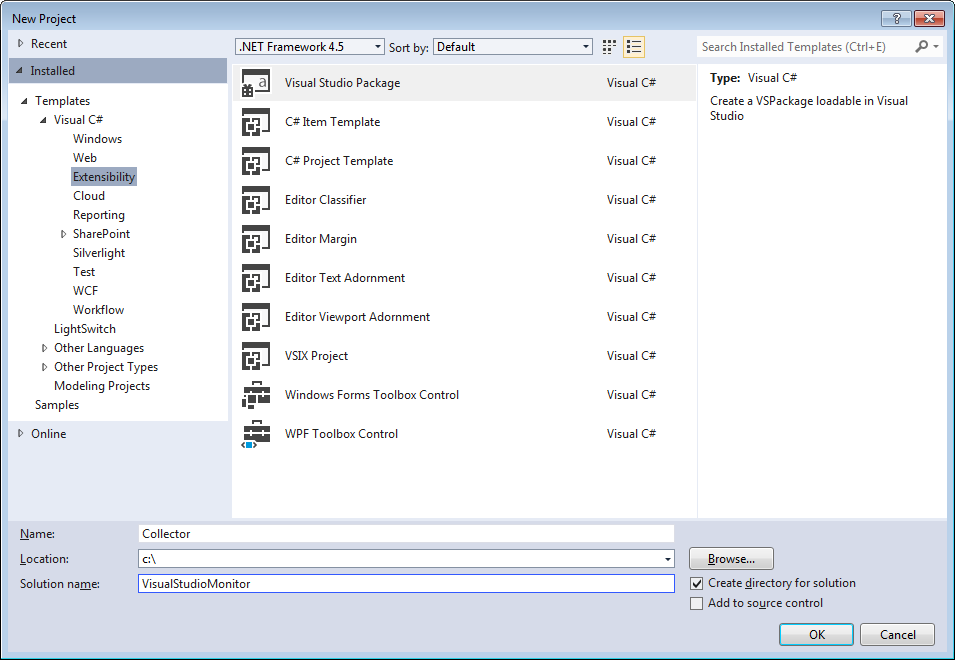
\includegraphics[width=4in]{CreateVSIXExtension.png}
	\caption{Create a Visual Studio Extension}
	\label{fig:ProjectCreation}
\end{figure}

For Name put "Collector" and Solution name put "VisualStudioMonitor", then follow the default options forthe first 2 steps of the wizard.  In the third step, when asked to specify what type of extension, click only the option to generate a menu command.  In the following step, give the menu command a name of "Stop Monitoring" and a command ID of "StopMonitoring".  This menu option will allow the user to halt collection of data if they wish without quitting Visual Studio.  Click next on the next step and then Finish to setup your extension solution project.

Next step is to instruct the extension package to load when Visual Studio starts. This is accomplished through an attribute set on the package class declaration for ProvideAutoLoad.  The file CollectorPackage.cs contains the class declaration for the extension package.   There are several optoins for when to load the package that are controlled by the GUID of the attribute.  Place the attribute as shown in the listing below before the package declaration.  This GUID will load the package when Visual Studio starts.

\begin{lstlisting}
    // This attribute starts the package when Visual Studio starts 
    [ProvideAutoLoad("{ADFC4E64-0397-11D1-9F4E-00A0C911004F}")]
    [Guid(GuidList.guidCollectorPkgString)]
    public sealed class CollectorPackage : Package
\end{lstlisting}

\item
After creating the project and solution, the solution explorer should look like figure \ref{fig:SolutionExplorer} showing the project files necessary for the extension to work.
\begin{figure}
	\centering
	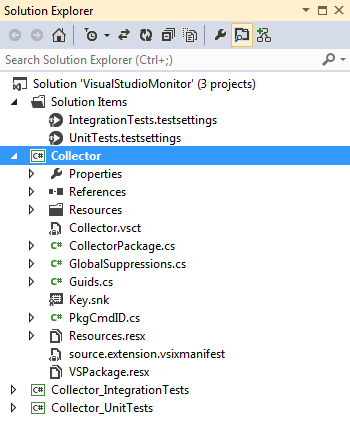
\includegraphics[width=2.5in]{SolutionExplorer.png}
	\caption{Solution Explorer with Visual Studio Extension}
	\label{fig:SolutionExplorer}
\end{figure}
\end{enumerate}

\subsubsection{Create Monitor Project}

\begin{enumerate}
\item
Good practice in extension development is to create a separate project (dll) for logic specific to the extension.  Add a class library type project to  the "Monitor" solution provide the data collection from Visual Studio and call it "Monitor".  the class library must be signed.  Go to the Properties for the Monitor project and select Signing from the list at the right.  In the Signing tab, check the "sign the assembly" checkbox then under "Choose a strong name key file", select Browse and browse over to the Key.snk file in the collector project (the file was created with the solution).
\item
The next step is to create a static class that will manage the log file including starting, stopping recording data, and inserting data into the log file.  Rename the class created by Visual Studio in the Monitor project to "DataRecorder".    Because we don't want more than one recorder running at a time and want to access this class without instantiating it, make the class static.  Create a method to Start the recorder that generates a file name for the log file and sets a flag that the recording has started. A Stop method resets that flag and perhaps clears the file name.  A method to write a log message to the file completes DataRecorder.
\item
Finally, insert a call to DataRecorder.Start() at the end of the Initialize() method in the CollectorPackage class.  This will start the monitoring each time Visual Studio starts.  You will need to add a reference for the "Monitor" project to the Collector project, make sure you sign the Monitor project, then rebuild the solution.


The call to DataRecorder.Start() is inserted in the CollectorPackage as shown in Listing \ref{code:StartCall}.
\begin{lstlisting}[caption=Call to DataRecorder.Start(),label=code:StartCall]
        /////////////////////////////////////////////////////////////////////////////
        // Overridden Package Implementation
        #region Package Members

        /// <summary>
        /// Initialization of the package; this method is called right after the package is sited, so this is the place
        /// where you can put all the initialization code that rely on services provided by VisualStudio.
        /// </summary>
        protected override void Initialize()
        {
            Debug.WriteLine (string.Format(CultureInfo.CurrentCulture, "Entering Initialize() of: {0}", this.ToString()));
            base.Initialize();

            // Add our command handlers for menu (commands must exist in the .vsct file)
            OleMenuCommandService mcs = GetService(typeof(IMenuCommandService)) as OleMenuCommandService;
            if ( null != mcs )
            {
                // Create the command for the menu item.
                CommandID menuCommandID = new CommandID(GuidList.guidCollectorCmdSet, (int)PkgCmdIDList.StopCollector);
                MenuCommand menuItem = new MenuCommand(MenuItemCallback, menuCommandID );
                mcs.AddCommand( menuItem );
            }
            DataRecorder.Start();
        }
        #endregion
\end{lstlisting}

The source code for the DataRecorder.cs file is shown in Listing \ref{code:DataRecorder}
\begin{lstlisting}[caption=Data Recorder Class,  label=code:DataRecorder]
using System;
using System.Collections.Generic;
using System.Linq;
using System.Text;
using System.Threading.Tasks;

namespace Monitor
{
    public static class DataRecorder
    {
        public static void Start() {
            logDirectoryPath = System.IO.Path.GetTempPath();
            logFileName = System.IO.Path.Combine(logDirectoryPath, "collector " + DateTime.Now.ToString("yyyy-MM-dd HH.mm.ss") + ".log");
            try {
                using (System.IO.StreamWriter streamWriter = new System.IO.StreamWriter(
                    new System.IO.FileStream(logFileName, System.IO.FileMode.OpenOrCreate, System.IO.FileAccess.Write, System.IO.FileShare.ReadWrite)
                    ))
                {
                    streamWriter.WriteLine("Collector Started");
                }
            } 
            catch (System.IO.IOException ioexception) {
                Console.WriteLine("Error creating log file "+ioexception);
            }
         }

        public static void Stop() {

                WriteLog("Collector Stopped");
            
        
        }

        public static void WriteLog(string logToWrite)
        {
            try
            {
                using (System.IO.StreamWriter streamWriter = new System.IO.StreamWriter(
                    new System.IO.FileStream(logFileName, System.IO.FileMode.Append, System.IO.FileAccess.Write, System.IO.FileShare.ReadWrite)
                    ))
                {
                    streamWriter.WriteLine(logToWrite);
                }
            }
            catch (System.IO.IOException ioexception)
            {
                Console.WriteLine("Error writing to log file " + ioexception);
            }
        
        }

        private static string logFileName;
        private static string logDirectoryPath;
    }
}

\end{lstlisting}
\end{enumerate}

\subsubsection{Create the Class Framework}

The next step creates a framework for storing and managing event monitoring for Visual Studio.  Because there are several different types of events, it makes sense to build an abstract class to manage the core data and use the Simple Factory pattern to generate each type of event monitoring.  With this pattern an abstract base class, called AbstractMonitoredEvent, provides common definitions for class fields that will be used for monitoring different Visual Studio events, conversion of those fields to and from the storage format, and (eventually) calling the WriteLog method in the recorder when the event fires.  This concrete class implements methods specific to Visual Studio commands that manages the fields available from the DTE.Command class.  The client in the Simple Factory pattern is a class that maintains the collection of events that either gets read from the file or queried from Visual Studio.   In this step we focus on the elements needed to store event information, and manage the configuration file data in XML format.

\begin{enumerate}
\item
Create the AbstractMonitoredEvent class in the Monitor project in Visual Studio.  Then add data elements for EventName and Classification as follows.

\begin{lstlisting}
    [XmlInclude(typeof(MonitoredCommandEvent))]
    [XmlRoot(ElementName = "MonitoredEvent", Namespace = "http://Monitor")]
    public abstract class AbstractMonitoredEvent
    {
        /// <summary>
        /// Default constructor to use in serialization
        /// </summary>
        protected AbstractMonitoredEvent()
        {
        }

        public String EventName { get; set; }
        public String Classification { get; set; }
   }
\end{lstlisting}

So that we can store events in a configuration file then manipulate that configuration file later, we provision this abstract class for XML serialization of itself and its derived classes.  Dot NET attributes support the XML serialization in this structure.  The first attribute tells XML serialization that the MonitoredCommandEvent class is a derived class of AbstractMonitoredEvent that we will create next.  This provides the abiltiy to serialize and deserialize the public objects of the derived class by referencing the type of AbstractMonitoredEvent when creating a serializer.  The second attribute creates an XML namespace that all derived classes will share with the AbstractMonitoredEvent class.

\item
The next step is to create a derived class called MonitoredCommandEvent that inherits from AbstractMonitoredEvent.  MonitoredCommandEvent implements a constructor that builds a MonitoredCommandEvent object from the Command class of the DTE and a constructor that builds from an XElement.  An output method ToXElement translates the object to XML for saving.

After you create the class, add using statements for System.Xml.Serilization, and EnvDTE and their corresponding references in the project References configuration. 

The EnvDTE.Command object contains fields for Guid (a GUID string), ID and integer sub-id, and Name a readable name for the command.  To register an event handler for a EnvDTE.Command, you need get an object reference for the command using the Guid and ID to identify the command.  The GUID is  a Globally Unique IDentifier for command events in Visual Studio, however, some command events share a GUID and distinguish themselves with different EventIDs. Thus both elements are necessary to link a Command event from the DTE to an event hander in this extension.  The Name is useful information to understand what the command is.    There are several versions of the DTE object corresponding to versions of Visual Studio.  Depending on the commands of interest, each version may need to be queried for its commands.  

 The constructor that takes a Command as input, simply extracts the necessary and relevant fields from the DTE's Command object and transferrs the matching information into the corresponding fields from this class and the AbstractMonitoredEvent class.  


\begin{lstlisting}
    [XmlRoot(ElementName = "MonitoredEvent", Namespace = "http://Monitor")]
    public class MonitoredCommandEvent : AbstractMonitoredEvent {

         public int EventID { get; set; }
        public String Guid { get; set; }

        public MonitoredCommandEvent()
        {
        }

        public MonitoredCommandEvent(Command DTECommandObj) {
            if (DTECommandObj != null) {
                this.EventName = DTECommandObj.Name;
                this.Classification = EventName.Split('.')[0];  //use the first part of event name
                this.Guid = DTECommandObj.Guid;
                this.EventID = DTECommandObj.ID;
            }
            else {
                throw new ArgumentNullException("DTECommandObj");
            }
        }
\end{lstlisting}

 The attribute for XMLRoot is the same attribute assigned to the AbstractMonitoredEvent class which tells XML Serialization that this type is a type beloging to the abstract class.  In this class, create two public fields, EventID as int and GUID as string, that will save important information from the Visual Studio DTE object needed to engage monitoring for each command.  

\item
To complete the Simple Factory pattern, a static factory class provides static factory methods that creates an object of type  MonitoredCommandEvent from a DTE Command object and returns it as an AbstractMonitoredEvent.  For now the only class to consider is the MonitoredCommandEvent derived class, however, a future step will add more derived classes.  
\end{enumerate}

\subsubsection{Query Save and Retrieve Visual Studio Command Event Info}

\begin{enumerate}
\item
In this step, build the MonitoredEventCollection class that manages a List object of AbstractMonitoredEvent type.  The List object gets populated from an XML file that stores the configuration data.  The MonitoredEventCollection class provides a method to query the DTE for all commands and initialize the list.  Another method called after the DTE query stores the List contents in the same XML format file.  These two methods should be called in sequence the first time the extension launches. After that, it  reads the XML file on startup to initialize the List.  Call the method(s) to query, store and load the event list from the Start() method of the DataRecorder class in the previous step so that the Monitor will load the commands on startup.

Fortunately the DTE object has a query method that lists all the commands it manages.   The DTE Commands object returns an IEnumerable collection of EnvDTE.Command objects. The listing below provides a method to try to get an instance of the DTE.  It depends on references to EnvDTE, Microsoft.VisualStudio.Shell.12.0, and Microsoft.VisualStudio.OLE.Interop so be sure to add those to the project's References list.

%\begin{lstlisting}[caption=Method to get a DTE Reference,label=code:tryGetDTEObject,float=ht]
\begin{lstlisting}

		using EnvDTE;
		using Microsoft.VisualStudio.Shell; //12.0
		private static DTE tryGetDTEObject()
		{
			DTE dteobj=null;
			try
			{
				dteobj = ((EnvDTE.DTE)ServiceProvider.GlobalProvider.GetService(typeof(EnvDTE.DTE).GUID)).DTE;

			}
			//Important to catch the following exception if the DTE object is unavailable
			catch (System.Runtime.InteropServices.InvalidComObjectException)
			{} 
			//Important to catch the following exception if the DTE object is busy
			catch (System.Runtime.InteropServices.COMException)
			{}
			return dteobj;
		}

\end{lstlisting}

Once you have a reference to the DTE object from the tryGetDTEObject method, use the DTE to query the Commands  object.  Then process each command into the List managed by MonitoredEventCollection.  Example code to do this is shown below making use of the MonitoredEventFactory to generate each AbstractMonitoredEvent stored in the List.  The try-catch here is necessary because the saved DTE object could get disposed while the loop proceses the Commands.

\begin{lstlisting}
                try
                {
                    foreach (Command DTE_CommandEventObj in dteobj.Commands)
                    {
                        AbstractMonitoredEvent NewEvent = MonitoredEventFactory.GetMonitoredEvent(DTE_CommandEventObj);
                        if (NewEvent != null)
                        {
                            EventList.Add(NewEvent);
                        }
                    }
                }
                //This exception happens during dispose/finalize when VS exits, just return null
                catch (System.Runtime.InteropServices.InvalidComObjectException)
                {
                    return null;
                }
\end{lstlisting}

\item
A persistent configuration file helps independently manage the events that get monitored for a study, and makes the configuration of all possible events easier to manage.    Using the framework's ToXelement methods, build methods in MonitoredEventCollection to save the List of AbstractMonitoredEvents to the configuration file and load them from the configuration file.  Below is the core code for the save to XML method that creates a serializer for the List object then writes that to the file stream.  Code for reading the XML file is left to the reader.

\begin{lstlisting}
                var serializer = new System.Xml.Serialization.XmlSerializer(typeof(List<AbstractMonitoredEvent>));
                using (Stream file = new FileStream(filepath, FileMode.Create, FileAccess.Write))
                {
                    serializer.Serialize(file, eventList);
                    file.Flush();
                }
\end{lstlisting}

\end{enumerate}


\newpage



\subsubsection{Register Event Handlers}

Now that the framework is complete and a configuration file for all command events to be monitored is ready, the methods to hook Visual Studio into event handlers that log each command can be created.  This step will add methods and member objects to AbstractMonitoredEvent and MonitoredCommandEvent classes to register event handlers with the DTE and dispose of them appropriately when necessary.  The MonitoredEventCollection class gets a new method to perform the registration from the objects in the list and another method to deregister them.

\begin{enumerate}
\item
The AbstractMonitoredEvent class should get a virtual RegisterEventForMonitoring method that takes an object parameter we will use to pass a DTE reference in.  The method returns a bool based on successful regisration.  The class also gets a non virtual Dispose() method  and a virtual Dispose(bool disposing) method with the former calling the latter and the latter setting a field isDisposed to true. This is the typical dispose structure.  Finally, the abstract class holds the non-virtual method to write the event log information (the abstract class's fields and a timestamp) to the log via the DataRecorder class.  This unifys logs for all derived classes into a common format.

\item
The MonitoredCommandEvent class overrides the virtual RegisterEventForMonitoring method to implement registering an event handler for Command events.  Registering first must find the event in the DTE and assign it to the field, then attach a new event hander to the event.  Looking at the method listing below, the Guid and EventID are used as parameters to query the DTE Events object for the specific command event in this instance.  The result is assigned to a field, eventTypeObject.  Wiith this reference to the event, the next block adds an event handler that runs after the command is executed.  After all that if the eventTypeObject is not null, the method returns true for success.
\begin{lstlisting}
        public override bool RegisterEventForMonitoring(object dte)
        {
            if (!isDisposed && eventTypeObject == null && dte != null)
            {
                eventTypeObject = (dte as DTE).Events.get_CommandEvents(Guid, EventID) as CommandEvents;
            }
            if (eventTypeObject != null)
            {
                eventTypeObject.AfterExecute += new 
			_dispCommandEvents_AfterExecuteEventHandler(OnAfterExecute);
            }
            return (eventTypeObject != null);
        }
\end{lstlisting}

With the above method in Visual Studio, the missing fields and methods can be auto-generated via the "Generate" context menu command.  

The last step with MonitoredCommandEvent is to create the Dispose method that will deregister the event handler. This looks like the following:

\begin{lstlisting}
        protected override void Dispose(bool disposing)
        {
            if (eventTypeObject != null) 
		eventTypeObject.AfterExecute -= OnAfterExecute;
            this.isDisposed = true;
        }
\end{lstlisting}

Use the Visual Studio "Generate" command to generate a method stub for OnAfterExecute and the
code will compile.  In the OnAfterExecute method, call ToLog so the event data is captured in the log.

\item
MonitoredEventCollection now needs methods to perform registration and deregistration on all the events in the list.  As the following listing shows, RegisterEventInventoryForEventMonitoring() must get the DTE object then walk through the IDEEventListenerRegistry list calling the abstract method RegisterEventForMonitoring with the DTE.  If one of them succeeds then this method considers it successful.

\begin{lstlisting}
        public bool RegisterEventInventoryForEventMonitoring()
        {
            DTE dteobj = tryGetDTEObject();
            bool somethingRegistered = false;
            if (dteobj != null && IDEEventListenerRegistry != null && IDEEventListenerRegistry.Count > 0)
            {
                foreach (AbstractMonitoredEvent command in IDEEventListenerRegistry)
                {
                    if (command.RegisterEventForMonitoring(dteobj))
                    {
                        somethingRegistered = true;
                    }
                }
            }
            return somethingRegistered;
        }
\end{lstlisting}

The method in MonitoredEventCollection to de-register events in the List via Dispose() is left as an exercise for the reader to complete.

\item
Refactor the MonitoredEventCollection object in DataRecorder to a static class field.  Then add a call to RegisterEventInventoryForEventMonitoring() in the Start() method of DataRecorder.  Add a call to the de-register method of MonitoredEventCollection in the Stop() method of DataRecorder.  

\item
Run the solution and use a few commands in Visual Studio, then give the Stop Collector command and check the log file.  You should see output like the following:
\begin{verbatim}
Collector Started
2014-02-02 13:46:52Z,Tools.AddinManager,Tools
2014-02-02 13:46:56Z,Tools.ExtensionsandUpdates,Tools
Collector Stopped
\end{verbatim}


\end{enumerate}


Below are descriptions of the code listings for the example code we discussed in this section.  Code listings are located at the end of the chapter.
\begin{itemize}
\item
The Listings for AbstractMonitoredEvent.cs in Code Listing \ref{code:AbstractMonitoredEvent_4}  show the additions to that class.  
\item
The listing for CommandMonitoredEvent.cs in Code Listing \ref{code:MonitoredCommandEvent_4} shows methods implemented for registration and disposal.
\item
The listing for MonitoredEventCollection.cs in Code Listing \ref{code:MonitoredEventCollection_4} shows list processing in calls to respective registration and de-registration methods for the List object.
\item
The DataRecorder class is shown in listing \ref{code:DataRecorder_4}.
\end{itemize}



\subsection{Classification of Events}
Now that the data collector is working, let's look at the classification of commands in Visual Studio according to the goal of understanding structured vs. unstructured navigation commands.  If you look at the generated XML file from MonitoredEventCollection, there are literally four thousand commands to choose from.  The sample program generates a base classification from the command family (usually a menu association), however, that does not distingush between navigation types.    The navigation events of interest relate to the prior stated metric Navigation Ratio.  For this metric,  we identify the  commands related to structured navigation (in Visual Studio) as follows:
\begin{itemize}
\item
 Navigate To (Ctrl+,) is a fuzzy search interface that lists identifiers matching the selected string
\item Go To Definition (F12) brings up the code that defines the selected identifier
\item View Call Hierarchy (Ctrl+K Ctrl+T) provides a two way analysis of an identifier's dependencies and uses
\item Class View (Ctrl+W, C) provides a browser and search function for classes and class hierarchy
\item Find All References (Ctrl+K,R) provides a list of lines that reference an identifier
\item Navigate to Event Handler in the XAML editor shows the event handler for an object
\item View Class Diagram generates a class diagram
\item View Object Browser is a search tool and browser
\end{itemize}

Next we identify the commands related to unstrctured navigation as follows:
\begin{itemize}
\item selecting a file in an explorer window
\item selecting the tab for a file
\item using arrow and page up/down keys to go up/down through a file
\item scrolling,
\item clicking on a file element
\item using GoTo Line command
\item using Find In Files command
\item using Quick Find command
\end{itemize}

These identified commands form the set of actions that usage data needs to collect to calculate the navigation ratio metric.  Notice that the commands are a mixture of defined actions within the tool and actions that result from mouse actions such as selecting a window or a window tab.  Now in the classification file generated from the tool, there is a field to classify each event.  Locating the events in the xml related to these commands and changing their classification to StructuredNav or UnstructuredNav will allow analaysis of the log data with respect to these classifications.

\subsubsection{Wrap Up}

With this demonstration you see how to build a usage monitor for Visual Studio that records most commands the user can issue in the IDE.  What's missing?  Well there are other areas of the DTE to explore such as editor events, unit test events, build and debug session events that provide greater context to the user experience.  For brevity, capturing those events is left to the reader to explore on their own.

%\subsubsection{Unstructured Navigation Events}
%For this step, an important set of code is added to Monitor so users unstructured navigation actions can be captured.  Since unsturcutured navigation includes actions like scrolling through a soruce file or opening a source file from a project browser, the event collection requires a different part of the Visual Studio DTE api.  

%Add a reference to EnvDTE80 to get access to this portion of the API.  

%Add a reference to Microsoft.VisualStudio.TextManager.Interop to get access to the text editor manager.


